%%%%%%%%%%%%%%%%%%%%%%%%%%%%%%%%%%%%%%%%%%%%%%%%%%%%%%%%%%%%%%%%%%%%%%
% How to use writeLaTeX: 
%
% You edit the source code here on the left, and the preview on the
% right shows you the result within a few seconds.
%
% Bookmark this page and share the URL with your co-authors. They can
% edit at the same time!
%
% You can upload figures, bibliographies, custom classes and
% styles using the files menu.
%
%%%%%%%%%%%%%%%%%%%%%%%%%%%%%%%%%%%%%%%%%%%%%%%%%%%%%%%%%%%%%%%%%%%%%%

\documentclass[12pt]{article}

\usepackage{sbc-template}

\usepackage{graphicx,url}
\usepackage{mathtools}
%\usepackage[brazil]{babel}   
\usepackage[utf8]{inputenc}  
\usepackage{booktabs}
\usepackage{listings}
\lstset{language=C++,
tabsize=4,
 breaklines=true,}

\sloppy

\title{Trabalho Prático\\Projeto e Análise de Algoritmos}

\author{Daniel Gunna Santana da Silva Souza,  Jordan Grangeiro Marinho Junior}

\address{ Pontíficia Universidade Católica de Minas Gerais  (PUC Minas) -- \\Instituto de Ciências Exatas e Informática - \\Ciência da Computação - Projeto e Análise de Algoritmos
}

\begin{document} 

\maketitle

     
\begin{resumo} 
  O Algoritmo de Dijkstra pode ser utilizado para encontrar o menor caminho entre dois vértices em um grafo,desde de que o  peso nas arestas seja positivo. Quando o objetivo é trabalhar com grafos que possuem arestas com pesos negativos, outra solução deve ser utilizada, pois o algoritmo proposto por Dijkstra trabalha apenas com arestas de pesos positivos, sendo assim, deve-se utilizar  outro algoritmo que use uma abordagem diferente, pois o proposto por Dijkstra torna-se ineficiente na reolução do problema. Trabalhou-se com o algoritmo de Bellman-Ford para a resolução do problema de grafos com arestas de pesos negativos, que trouxe resultados que mostram a eficiência do algoritmo neste tipo de situação.
\end{resumo}


\section{Introdução}

Nesse trabalho, analisou-se o uso do algoritmo de Dijkstra para grafos com arestas
de peso não negativos, e uma possível solução para grafos com arestas de pesos negativos. O algoritmo de 
Dijkstra procura encontrar o menor caminho em um grafo, dirigido ou não,
sem conter arestas de peso negativo. Uma solução para o problema das arestas negativas seria o uso do algoritmo
de Bellman-Ford. O algoritmo de Bellman-Ford também será utilizado, como abordagem para a resolução do problema de determinar a existência de um Ciclo Negativo em um grafo. Ambos os algoritmos e os problemas que eles se propõe a resolver   serão discutidos de maneira mais detalhada no decorrer do artigo.

\section{Implementação} \label{sec:implementacao}
A codificação dos algortimos abordados neste trabalho foi realizada   utilizando a linguagem de programação C++, através do editor de texto padrão do Sistema Operacional Ubuntu 14.04, o gedit   juntamente com o software de edição de texto Geany. Os códigos foram compilados usando o compilador GNU G++ 4.8.4, que já vem por padrão com o Ubuntu.A linha de comando utilizada no terminal padrão do Ubunutu, o Consola, para compilação seguiu o seguinte padrão: \textit{\$ g++ nomePrograma.c -o nomePrograma}. Para as execuções, após a compilação, utilizou-se o comando: \textit{\$ ./nomePrograma}.
\\Para a codificação  dos algoritmos discutidos no trabalho, fez-se necessária a utilização das seguintes estruturas de dados e definições:

\begin{enumerate}
\item \textbf{\#define} V
\\
V é definido com a quantidade de vértices que grafo a ser usado possuirá.
\\
\item \textbf{int} grafo[V][V]
\\
A estratégia abordada para representação do Grafo foi usar uma matriz de adjacências, onde uma dada posição i,j da matriz conterá o peso da aresta que incide nos vértices i e j,caso exista aresta entre eles. A matriz abstraída do grafo será uma  matriz de inteiros  de dimensão VxV.
\\
\item \textbf{int} distancia[V]
\\
distancia[i] guardará a menor distância do vértice \textit{src} até o vértice i. Inicialmente inicializado como infinito para todas as posições.
\\
\end{enumerate}

\subsection{Algoritmo de Dijkstra} \label{sec:dijkstra}

O algoritmo de Dijkstra proposto em \cite{Dijkstra1959} soluciona o problema do caminho mais curto em grafos de 
pesos não negativos. O algoritmo está inserido no paradigma de progamação denominado como algoritmos gulosos, pois o algoritmo  realiza uma
comparação entre todos os vértices adjacentes ao vértice analisado para  escolher o que parece melhor, ou seja, possui aresta de menor peso, assim passando por todos os vértices do grafo e encontrando o caminho mais
curto. Este comportamento do algoritmo possui uma  das características do paradigma dos algoritmos gulosos, que é: para resolver um problema escolher o melhor resultado conhecido que se encontra disponível, independentemente das próximas iterações.
A implementação se resume em algumas estruturas de dados e duas principais funções:
 
\begin{enumerate}
\item \textbf{bool} visitado[]
\\
Estrutura de dados para armazenar quais vértices do grafo já foram visitados pelo algoritmo. O valor em v[i] será igual a \textit{true} se o vertice i já foi visitado e \textit{false} caso contrário. O acesso a visitado[i]  nos diz se o vértice i ja foi visitado. Inicialmente toda a estrutura de dados é  inicializada com \textit{false} para todas as posições.
\\
\item \textbf{void} dijkstra(\textbf{int} grafo[V][V], \textbf{int} src)
\\Procedimento  que implementa  "o fluxo  principal" do algoritmo de Dijkstra. Itera sobre todos os vértices do grafo, encontrando, para cada vértice, o vértice \textit{u} de menor distância em relação ao \textit{src}(vértice origem), utilizando o valor inteiro retornado pela    função \textit{int distanciaMin(distancia[], visitado[])}. Escolhido esse vértice \textit{u}, realiza-se uma iteração sobre os vértices adjacentes a \textit{u}, atualizando os valores do arranjo de distâncias, respeitando às seguintes condições e restrições:
\begin{itemize}
\item O vértice \textit{v} não pode ter sido visitado;
\item Existir uma aresta entre \textit{u} e \textit{v};
\item Peso total do caminho entre o vértice origem (\textit{src}) e \textit{v} for menor que o valor da distância na iteração corrente;
\end{itemize}
\item \textbf{int} distanciaMin(\textbf{int} distancia[], \textbf{bool} visitado[])
\\
Função auxiliar, que encontra o vértice com a menor distância em relação ao \textit{src}(vértice origem)  no conjunto de vértices ainda não incluídos na árvore de menor caminho. Recebe como parâmetro o arranjo de distâncias, e o arranjo de vértices  de visitados.
\end{enumerate}

Após  a  execução do algoritmo, o programa retorna o aranjo de distâncias que contém a distância de cada vértice do grafo  para o vértice \textit{src}, definido como vértice origem  origem.


\subsection{Algoritmo de Bellman-Ford}\label{sec:bellman-ford}

O algoritmo de Dijkstra se limita a grafos que possuam apenas  arestas de peso  positivo. Isso se deve ao fato do algoritmo  assumir  como distância minima entre dois vértices adjacentes, o peso da aresta entre esse dois vértices, caso exista. Uma heurística criada  para resolver esse problema seria a adição de uma constante \textit{X} ao peso de todas as arestas do grafo, de forma a garantir que todas as arestas sejam positivas.Porém um problema dessa abordagem é a escolha dessa constante, que, caso seja escolhida de maneira errada, pode anular alguma aresta e, consequentemente, atrapalhar o fluxo original do grafo.
\\O algoritmo de Bellman-Ford foi proposto por Shimbel em 1955, publicado por Richard Bellman e Lester Ford, Jr. em 1958. É um algoritmo mais  lento em sua execução e com custo computacional que pode ser superior  se comparado com  o Algoritmo de Dijsktra, quando usado para resolver o mesmo problema,porém  mas é mais versátil e robusto por ser capaz de executar a busca do caminho minimo para dígrafos, com arestas de pesos negativos. A implementação do Algortimo de Bellman Ford se resume em um único método  principal:

\begin{itemize}
\item \textbf{void} BellmanFord(\textbf{int} grafo[V][V], \textbf{int} src)\\ 
Realiza-se uma iteração  sobre todos os vértices do grafo, encontrando, para cada vértice, o vértice \textit{u} de menor distância em relação ao \textit{src}(vértice origem), respeitando às seguintes condições e restrições:
\begin{itemize}
\item Deve existir uma aresta entre os vértices correntes na iteração;
\item Peso total do caminho entre \textit{src}(vértice origem) e \textit{v} for menor que o valor da distância na iteração corrente;
\end{itemize}
\end{itemize}
Diferentemente do Algoritmo de Dijkstra, o Algoritmo de Bellman Ford está inserido no paradigma de programação dinâmica.
Como em outros problemas de programação dinâmica, o algoritmo calcula os menores caminhos de maneira \textit{bottom-up}, ou seja, construindo soluções de porções menores do problema, armazenando-as em uma estrutra, e posteriormente utilizando a soluções já computadas e  armazenadas para construir  as próximas soluções. O algoritmo primeiramente calcula as menores distâncias para os menores caminhos que possuam no máximo 1 aresta no caminho. A partir disso, calcula-se nas próximas iterações para 2, 3, ..., \textit{i} arestas. Após isso, iterando sobre todas as arestas garantimos encontrar o menor caminho, com os valores anteriores já calculados e armazenados  no início do algoritmo.

\subsubsection{Ciclo Negativo}
Para a determinarmos a exitência de ciclos negativos no grafo, deve-se realizar uma interação  novamente por todos os vértices, logo após a execução da função \textit{void BellmanFord(...)}, através da função \textit{\textbf{void} hasCicloNegativo(\textbf{int} grafo[V][V], \textbf{int} distancia[])} verificando as seguintes condições e restrições para determinar a solução:

\begin{enumerate}
\item Deve existir aresta entre os dois vértices na iteração corrente;
\item Distancia do vértice da iteração interna até o \textit{src}(vértice origem) for diferente de infinito;
\item Distancia do vértice da iteração interna até o \textit{src}(vértice origem) + o peso da aresta entre os dois vértices correntes for menor que a distância do vértice da iteração interna.
\end{enumerate}

A função irá mostrar na tela a mensagem  \textit{TRUE} caso exista ciclo negativo no grafo, ou mostrar \textit{FALSE} caso o grafo não possua ciclo negativo.




\section{Análise de complexidade }
Seja a operação relevante para todos os algoritmos citados neste trabalho a comparação entre os elementos do vetor.
\subsection{Dijkstra  \(\Rightarrow\) \(\Theta(V^{2})\)}
\begin{itemize}
\item Melhor caso = Pior caso:
\subitem \textbf{void} dijkstra(\textbf{int} grafo[V][V], \textbf{int} src) \(\Rightarrow\) \(\Theta(V^{2})\) : È bem simples observar isto analisando-se o algoritmo implementado, pois basta apenas observar que deve-se percorrer a matriz de dimensão VxV, realizando as comparações para cada vértice.
\subitem  \textbf{int} distanciaMin(\textbf{int} distancia[], \textbf{bool} visitado[]) \(\Rightarrow\) \(\Theta(V)\) :Também é bastante trivial observa isso analisando-se o a implementação, pois este procedimento percorrer todos os V vértices do grafo buscando pelo vertice não visitado de disitância minima.
\\
%\item OBS:  Existe uma implementação do Algoritmo de Dijkstra, utilizando uma fila de prioridades 
\end{itemize}


\subsection{Bellman-Ford  \(\Rightarrow\) \(\Theta(V^{2})\)} 

\begin{itemize}
\item Melhor caso = Pior Caso:
\subitem \textbf{void} BellmanFord(\textbf{int} grafo[V][V], \textbf{int} src) \(\Rightarrow\) \(\Theta(V^{2})\) : Analisando-se a implementação do algoritmo observa-se que para cada vértice existente na matriz de dimensão VxV, deve-se  verificar se existe aresta, se não existe caminho entre o vértice atual e o fonte e se o caminho encontrado é menor do que o armazenado no arranjo de distâncias. Sendo assim para cada vertice  u que iteramos  devemos realizar estas comparações  iterando  em todos os vértices  v do grafo, chegando assim a complexidade encontrada.
			

\end{itemize}

\subsection{Bellman-Ford para ciclo negativo  \(\Rightarrow\) \(\Theta(V^{2})\)}


\begin{itemize}
\item Melhor caso = Pior caso:
\subitem \textbf{void} BellmanFord(\textbf{int} grafo[V][V], \textbf{int} src) \(\Rightarrow\) \(\Theta(V^{2})\)
\subitem  \textbf{int} hasCicloNegativo(\textbf{int} grafo[V][V], \textbf{int} distancia[]) \(\Rightarrow\) \(\Theta(V^{2})\)
\end{itemize}


\section{Testes}


Foram realizados testes utilizado-se  os três algoritmos. Em todos os algoritmos testados,  as entradas utilizadas como instâncias do problema foram os grafos 01, 02 e 03 ilustrados na Figure 1.

\begin{figure}[!htb]
\centering
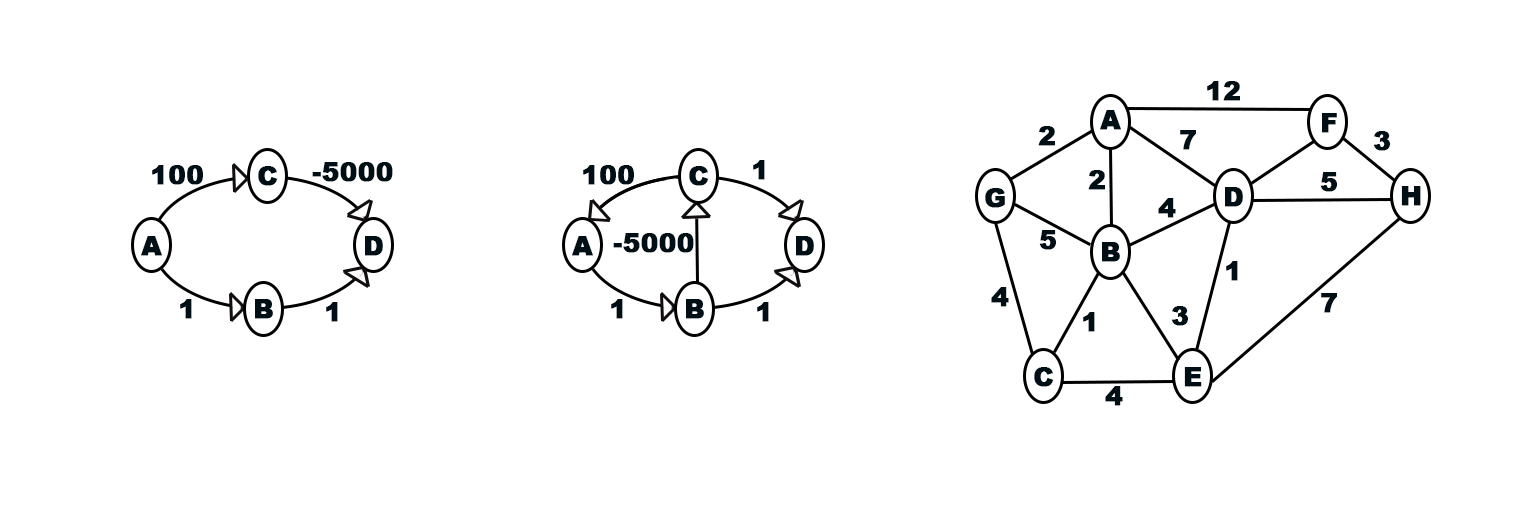
\includegraphics[scale=0.3]{Grafos.png}
\caption{Grafos 1, 2 e 3 respectivamente.}
\label{Rotulo}
\end{figure}


\subsection{Saídas do Algoritmo de Dijkstra}
Analisando as saídas  das tabelas 1, 2 e 3, observamos que o algoritmo nos retorna a menor distância a ser percorrida de um vértice inicial \textit{src} para todos os vértices existentes no grafo. As tabelas 1 e 2, que mostram as saídas produzidas pelo algoritmo de Dijkstra para os grafos 01 e 02, nos mostram a deficiência do algoritmo de Dijkstra em operar em grafos com  arestas de peso negativo. Isto ocorre devido ao fato de que em sua execução, são analisados todos os vértices adjacentes ao vértice atual e sendo assim, de certa forma, o algoritmo considera que é impossível que exista uma outra forma de se chegar ao vértice adjacente ao analisado, de maneira que o caminho seja menor que o peso da aresta entre esses dois vértices, uma vez que este peso é negativo.
\begin{table}[h!]
  \centering
  \caption{Saída Grafo 01 - Algoritmo de Dijkstra}
  \label{tab:table1}
  \begin{tabular}{ccc}
    \toprule
    Vértice & Distância para o vértice fonte (A)\\
    \midrule
    A & 0\\
    B & 1\\
    C & 100\\
   D & 2\\
    \bottomrule
  \end{tabular}
\end{table}

\begin{table}[h!]
  \centering
  \caption{Saída Grafo 02 - Algoritmo de Dijkstra}
  \label{tab:table1}
  \begin{tabular}{ccc}
    \toprule
    Vértice & Distância para o vértice fonte (A)\\
    \midrule
    A & 0\\
    B & 1\\
    C & -4999\\
   D & -4998\\
    \bottomrule
  \end{tabular}
\end{table}

\begin{table}[h!]
  \centering
  \caption{Saída Grafo 03 - Algoritmo de Dijkstra}
  \label{tab:table1}
  \begin{tabular}{ccc}
    \toprule
    Vértice & Distância para o vértice fonte (A)\\
    \midrule
    A & 0\\
    B & 2\\
    C & 3\\
    D & 6\\
    E & 5\\
     F & 12\\
      G & 2\\
       H & 11\\
    \bottomrule
  \end{tabular}
\end{table}

\subsection{Saídas do Algoritmo de Bellman-Ford}
A partir dos resultados mostrados nas tabelas 4, 5 e 6, é possível perceber a grande diferença, comparando com com os resultados obtidos por Dijkstra, especificamente os resultados das saídas para  os grafos 01 e 02. Isto se deve à forma como o Algoritmo de Bellman-Ford resolve o problema, permitindo arestas de peso  negativo e calculando de maneira correta o menor caminho, considerando as mesma. Porém o   algoritmo é mais lento quando comparado ao Dikjstra, isso se deve pelo  fato que este algoritmo deve  analisar a distância entre todos os vértices do grafo, para eliminar a possibilidade de erro com arestas de peso negativo encontradas nas saídas do Algoritmo de Dijkstra. Entretando, utiliza de uma abordagem sofisticada de Programação Dinâmica, na qual guarda-se o cálculo das distãncias entre os vértices que podem ser necessárias  posteriormente, em uma estrutura de dados que é consultada para determinar cálculos  futuros.\\
Já as tabelas 7, 8 e 9 nos mostram as saídas poduzidas pelo algoritmo que determina a   existência de Ciclo Negativo. Observamos  como o algoritmo em questão trabalha de forma eficiente para determinar a solução, identificando a presença dos ciclos negativos, condizendo com os grafos de entrada apresentados  conforme Figure 1.

\begin{table}[h!]
  \centering
  \caption{Saída Grafo 01 - Algoritmo de Bellman-Ford}
  \label{tab:table1}
  \begin{tabular}{ccc}
    \toprule
    Vértice & Distância para o vértice fonte (A)\\
    \midrule
    A & 0\\
    B & 1\\
    C & 100\\
   D & -4900\\
    \bottomrule
  \end{tabular}
\end{table}

\begin{table}[h!]
  \centering
  \caption{Saída Grafo 02 - Algoritmo de Bellman-Ford}
  \label{tab:table1}
  \begin{tabular}{ccc}
    \toprule
    Vértice & Distância para o vértice fonte (A)\\
    \midrule
    A & -4899\\
    B & 1\\
    C & -4999\\
   D & 2\\
    \bottomrule
  \end{tabular}
\end{table}

\begin{table}[h!]
  \centering
  \caption{Saída Grafo 03 - Algoritmo de Bellman-Ford}
  \label{tab:table1}
  \begin{tabular}{ccc}
    \toprule
    Vértice & Distância para o vértice fonte (A)\\
    \midrule
    A & 0\\
    B & 2\\
    C & 3\\
    D & 6\\
    E & 5\\
     F & 12\\
      G & 2\\
       H & 11\\
    \bottomrule
  \end{tabular}
\end{table}

\begin{table}[h!]
  \centering
  \caption{Saída Grafo 01 - Algoritmo de Bellman-Ford - Ciclo negativo}
  \label{tab:table1}
  \begin{tabular}{ccc}
   \toprule
    Ciclo negativo & NAO\\
    \bottomrule
  \end{tabular}
\end{table}

\begin{table}[h!]
  \centering
  \caption{Saída Grafo 02 - Algoritmo de Bellman-Ford - Ciclo negativo}
  \label{tab:table1}
  \begin{tabular}{ccc}
    \toprule
    Ciclo negativo & SIM\\
    \bottomrule
  \end{tabular}
\end{table}

\begin{table}[h!]
  \centering
  \caption{Saída Grafo 03 - Bellman-Ford - Ciclo negativo}
  \label{tab:table1}
  \begin{tabular}{ccc}
    \toprule
    Ciclo negativo & NAO\\
    \bottomrule
  \end{tabular}
\end{table}

\section{Conclusão}
Neste trabalho concluímos que a melhor solução, entre as analisadas, para encontrar o menor caminho em grafos com arestas de peso negativo é o Algoritmo de Bellman-Ford. Concluímos que o Algoritmo de Bellman-Ford também é uma boa solução para determinar a existência de ciclos negativos em grafos.Observou-se também que mesmo o Algoritmo de Dijkstra sendo menos custoso em alguns casos e mais rápido, em alguns contextos de aplicação o Algoritmo de Bellman-Ford, é uma solução a ser considerada ao invés do Dijkstra, por sua  sofisticação e engenhosidade característa do Paradigma de Programação Dinâmica\cite{bellmandford} e facilidade de implementação, mesmo considerando algumas heurísticas combinadas ao Dijkstra para resolução do problema do menor caminho em grafos com arestas negativas.



\section{References}

Os algoritmos e definições trazidas neste trabalho foram baseadas nas referências citadas a seguir: \cite{zivianiprojeto}, \cite{cormen},
\cite{bellmandford}, and \cite{bellmand}

\bibliographystyle{sbc}
\bibliography{sbc-template}

\section{Anexos}
\subsection{Algoritmo de Dijkstra}




\begin{lstlisting}
// Dijkstra em C/C++ para encontrar o menor caminho
#include <stdio.h>
#include <limits.h>

// Numero de vertices do Grafo
#define V 9

// Funcao para encontrar o vertice de menor distancia entre o conjunto de vertices
// ainda nao visitados 
// nao incluido no conjunto de menor caminho
int distanciaMin(int distancia[], bool visitado[]){
   // Inicializa o valor minimo
   int min = INT_MAX;
   int min_index;
	//Percorrer o grafo procurando o vertice nao vistado
	//de menor distancia
	for (int i = 0; i < V; i++){
		if (visitado[i] == false && distancia[i] <= min){
			min = distancia[i];
			min_index =i;
		}
	}
    return min_index;
}

// Metodo p/ imprimir o array de distancia
void mostraSolucao(int distancia[], int n){
   printf("Vertice  Distancia do vertice fonte\n");
   for (int i = 0; i < V; i++){
      printf("%d \t\t %d\n", i, distancia[i]);
   }
}

// Implementacao do  Dijkstra, para matriz de adjacencia
void dijkstra(int grafo[V][V], int src){
     int distancia[V];  // Array para guardar a distancia mais curta entre src
						// e o vertice i 

     bool visitado[V];  // visitado[i] sera true se o vertice ja estiver incluido 
						// na arvore de menor caminho 

     // Inicializa a distancia de todos os vertice com  INFINITO 
	 //e false no array  visitados p/ todos os vertice
     for (int i = 0; i < V; i++){
        distancia[i] = INT_MAX, visitado[i] = false;
	 }

     // Distancia entre o vertice origem  e ele mesmo sempre sera 0
     distancia[src] = 0;

     // Encontra o menor caminho para todos os vertices
     for (int i = 0; i < V-1; i++){
		// Pega a menor distancia apartir do conjunto de vertices nao processados
		// u sempre possui o valor de src na primeira iteracao
		int u = distanciaMin(distancia, visitado);
       // Marca o vertice escolhido como visitado
       visitado[u] = true;
       // Atualiza o valor da distancia do vertice escolhido com os vertices adjacentes
       for (int j = 0; j < V; j++){
         // Atualiza a distancia[j] somente se ele nao foi visitado e 
		 // se existe uma aresta de u para j e 
		 // se o peso total do caminho da fonte para j passando por u e
		 // menor do que a distancia[j]
			if (!visitado[j] && grafo[u][j] 
						  && distancia[u] != INT_MAX 
						  && distancia[u]+grafo[u][j] < distancia[j]){
				distancia[j] = distancia[u] + grafo[u][j];
		
			}
		}
	}
     // Imprime o array de distancias
     mostraSolucao(distancia, V);
}

//Metodo principal
int main()
{
   // Grafo de exemplo
   int grafo[V][V] = {{0,  4,  0,  0,  0,  0,  0,  8,  0},
                      {4,  0,  8,  0,  0,  0,  0,  11, 0},
                      {0,  8,  0,  7,  0,  4,  0,  0,  2},
                      {0,  0,  7,  0,  9,  14, 0,  0,  0},
                      {0,  0,  0,  9,  0,  10, 0,  0,  0},
                      {0,  0,  4,  0,  10, 0,  2,  0,  0},
                      {0,  0,  0,  14, 0,  2,  0,  1,  6},
                      {8,  11, 0,  0,  0,  0,  1,  0,  7},
                      {0,  0,  2,  0,  0,  0,  6,  7,  0}};
	// Executa Dijkstra para o grafo acima
    dijkstra(grafo, 0);
    return 0;
}


 

\end{lstlisting}

\subsection{Algoritmo de Bellman-Ford}
\begin{lstlisting}
// Bellman-Ford em C/C++ para encontrar o menor caminho com arestas negativas
#include <stdio.h>
#include <stdlib.h>
#include <string.h>
#include <limits.h>

// Define o numero de vertices
#define V 4

// Metodo para imprimir a resposta
void mostraSolucao(int distancia[]){
    printf("Vertex   Distance from Source\n");
    int i;
    for (i = 0; i < V; ++i){
		printf("%d \t\t %d\n", i, distancia[i]);
	}
      
}

// Funcao para verificar se tem ciclo negativo e imprimir a resposta
bool hasCicloNegativo(int grafo[V][V], int distancia[]){
    bool resposta = false;
    // Se encontrar um caminho mais curto do que o ja salvo
    // e porque existe um ciclo negativo
    for (int u = 0; u < V; u++){
        for (int v = 0; v < V; v++){
            if (grafo[u][v] && distancia[u] != INT_MAX && distancia[u] + grafo[u][v] < distancia[v])
                resposta = true;
        }
    }
    return resposta;
}

// Metodo para encontrar a menor distancia entre o vertice oriem e
// todos os outros, usando o algoritmo de Bellman-Ford.
// O metodo   tambem detecta ciclos negativos
void BellmanFord(int grafo[V][V], int src){
    int distancia[V];
    int i, j;
    // Inicia o array de distancias entre o vertice fonte e todos os
	// outros com INFINITO
    for (i = 0; i < V; i++){
        distancia[i]   = INT_MAX;
	}
	// A distancia entre o vertice origem e ele mesmo e sempre zero
    distancia[src] = 0;
    
    // Passar por todos os vertices procurando o menor caminho entre o
	// vertice atual e o origem
    for (int u = 0; u < V; u++){
        for (int v = 0; v < V; v++){
			// Verifica se existe aresta, se nao existe caminho entre 
			// o vertice atual e o fonte e se o caminho encontrado e menor 
			// do que o armazenado no array de distancias. Se for
			// salvar o novo caminho
            if (grafo[u][v] && distancia[u] != INT_MAX && distancia[u] + grafo[u][v] < distancia[v]){
                distancia[v] = distancia[u] + grafo[u][v];
			}
        }
    }

	// Mostra a solucao do grafo com pesos negativos mas apenas se nao existir ciclos
	// negativos 
	if(!hasCicloNegativo){   
    		mostraSolucao(distancia);
	}else{
		printf("Contem Ciclo negativo - o programa sera encerrado\n");	
	}
    return;
}

// Metodo principal
int main(){    
    // Criando um grafo na matriz de adjacencia de exemplo
    int grafo[V][V] = {{0,   1,     0, 0},
					   {0,   0, -5000, 1},
		               {100, 0,     0, 1},
		               {0,   0,     0, 0}
    };
    
    // Executando o Bellman-Ford
    BellmanFord(grafo, 0);
    return 0;
}

\end{lstlisting}


\subsection{Algoritmo de Bellman-Ford - Ciclos Negativos}
\begin{lstlisting}
// Bellman-Ford em C/C++ para encontrar ciclos negativos
#include <stdio.h>
#include <stdlib.h>
#include <string.h>
#include <limits.h>

// Numero de vertices
#define V 4

// Metodo para verificar se tem ciclo negativo e imprimir a resposta
void hasCicloNegativo(int grafo[V][V], int distancia[]){
    bool resposta = false;
    // Se encontrar um caminho mais curto do que o ja salvo
    // e porque existe um ciclo negativo
    for (int u = 0; u < V; u++){
        for (int v = 0; v < V; v++){
            if (grafo[u][v] && distancia[u] != INT_MAX && distancia[u] + grafo[u][v] < distancia[v])
                resposta = true;
        }
    }
    if(resposta)
        printf("TRUE\n");
    else
        printf("FALSE\n");
}

// Metodo para encontrar o menor caminho entre o vertice fonte e
// todos os outros vertices, usando Bellman-Ford para detectar os
// ciclos negativos
void BellmanFord(int grafo[V][V], int src){
    int distancia[V];
    int i, j;
    // Inicializar o array de distancias entre o vertice fonte e todos os
    // outros com INFINITO
    for (i = 0; i < V; i++){
        distancia[i]   = INT_MAX;
    }
    // A menor distancia entre o vertice fonte e ele mesmo sempre sera zero
    distancia[src] = 0;
    
    // Verifica se o caminho encontrado e menor do que o armazenado no 
    // array de distancias, se for menor salva o novo caminho
    // Esse passo executa para pesos positivos
    for (int u = 0; u < V; u++){
        for (int v = 0; v < V; v++){
            if (grafo[u][v] && distancia[u] != INT_MAX && distancia[u] + grafo[u][v] < distancia[v]){
				distancia[v] = distancia[u] + grafo[u][v];
			}
                
        }
    }
    
    // Checar se existe um ciclo negativo. Como o passo acima so 
    // executa para pesos positivos, se encontrar um caminho mais 
    // curto e porque existe um ciclo negativo 
    hasCicloNegativo(grafo, distancia);
    return;
}

int main(){
    // Criando um grafo para exemplo
    int grafo[V][V] = {{0,  1,  100, 0},
                       {0,  0,    0, 1},
                       {0, -5000, 0, 0},
                       {0,  0,    0, 0}
    };
    // Executa o Bellman-Ford
    BellmanFord(grafo, 0);

    return 0;
}

\end{lstlisting}

\end{document}
